\documentclass[a4paper,5pt]{amsbook}
%%%%%%%%%%%%%%%%%%%%%%%%%%%%%%%%%%%%%%%%%%%%%%%%%%%%%%%%%%%%%%%%%%%%%

\usepackage{booktabs}
\usepackage{graphicx}
\usepackage{multicol}
\usepackage{textcomp}
\usepackage{systeme}
\usepackage{amssymb}
\usepackage[]{amsmath}
\usepackage{subcaption}
\usepackage[inline]{enumitem}
\usepackage{gensymb}

%%%%%%%%%%%%%%%%%%%%%%%%%%%%%%%%%%%%%%%%%%%%%%%%%%%%%%%%%%%%%%

\newcommand{\sen}{\,\mbox{sen}}
\newcommand{\tg}{\,\mbox{tg}\,}
\newcommand{\cosec}{\,\mbox{cosec}\,}
\newcommand{\cotg}{\,\mbox{cotg}\,}
\newcommand{\tr}{\,\mbox{tr}\,}
\newcommand{\ds}{\displaystyle}
\newcommand{\ra}{\rightarrow}

%%%%%%%%%%%%%%%%%%%%%%%%%%%%%%%%%%%%%%%%%%%%%%%%%%%%%%%%%%%%%%%%%%%%%%%%

\setlength{\textwidth}{16cm} %\setlength{\topmargin}{-1.3cm}
\setlength{\textheight}{25cm}
\setlength{\leftmargin}{1.2cm} \setlength{\rightmargin}{1.2cm}
\setlength{\oddsidemargin}{0cm}\setlength{\evensidemargin}{0cm}

%%%%%%%%%%%%%%%%%%%%%%%%%%%%%%%%%%%%%%%%%%%%%%%%%%%%%%%%%%%%%%%%%%%%%%%%

% \renewcommand{\baselinestretch}{1.6}
% \renewcommand{\thefootnote}{\fnsymbol{footnote}}
% \renewcommand{\theequation}{\thesection.\arabic{equation}}
% \setlength{\voffset}{-50pt}
% \numberwithin{equation}{chapter}

%%%%%%%%%%%%%%%%%%%%%%%%%%%%%%%%%%%%%%%%%%%%%%%%%%%%%%%%%%%%%%%%%%%%%%%

\begin{document}
\thispagestyle{empty}
\pagestyle{empty}
\begin{minipage}[h]{0.14\textwidth}
	
\includegraphics[scale=0.24]{../../ufgd.png}
\end{minipage}
\begin{minipage}[h]{\textwidth}
\begin{tabular}{c}
{{\bf UNIVERSIDADE FEDERAL DA GRANDE DOURADOS}}\\
{{\bf C\'alculo Diferencial e Integral III --- Lista 11}}\\
{{\bf Prof.\ Adriano Barbosa}}\\
\end{tabular}
\vspace{-0.45cm}
%
\end{minipage}

%------------------------

\vspace{1cm}
%%%%%%%%%%%%%%%%%%%%%%%%%%%%%%%%   formulario  inicio  %%%%%%%%%%%%%%%%%%%%%%%%%%%%%%%%
\begin{enumerate}
    \setlength\itemsep{0.5cm}
    \item Fa\c{c}a uma correspond\^encia entre as equa\c{c}\~oes param\'etricas e as curvas.

    \hspace{-1.5cm}
    \begin{minipage}[l]{0.5\textwidth}
        \begin{enumerate}
            \setlength\itemsep{0.2cm}
            \item $x=t\cos{t}, y=t, z=t\sen{t}, t\ge 0$
            \item $x=\cos{t}, y=\sen{t}, z=\cos{2t}$
            \item $x=\cos{8t}, y=\sen{8t}, z=e^{0,8t}, t\ge 0$
            \item $x=\cos^2{t}, y=\sen^2{t}, z=t$
        \end{enumerate}
    \end{minipage}
    \begin{minipage}[l]{0.5\textwidth}
        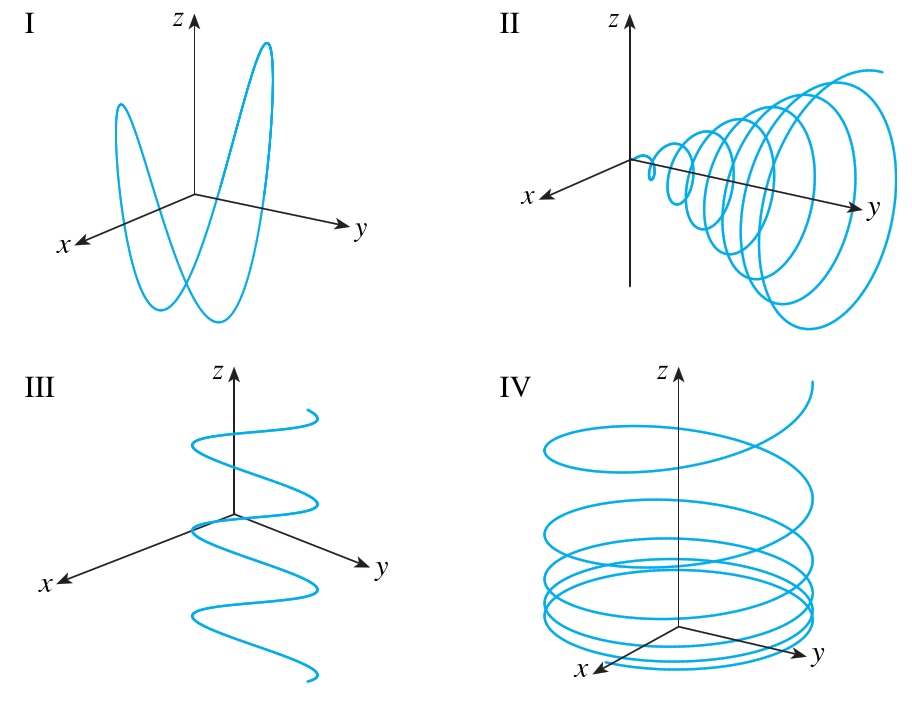
\includegraphics[width=\textwidth]{lista-11-fig2.png}
    \end{minipage}

    \item Fa\c{c}a a correspond\^encia entre os campos vetoriais e as figuras.

    \hspace{-1.5cm}
    \begin{minipage}[r]{0.4\textwidth}
        \begin{enumerate}
            \setlength\itemsep{0.2cm}
            \item $F(x,y) = (x,-y)$
            \item $F(x,y) = (y,x-y)$
            \item $F(x,y) = (y,y+2)$
            \item $F(x,y) = (\cos{(x+y)}, x)$
        \end{enumerate}
    \end{minipage}
    \begin{minipage}[l]{0.5\textwidth}
        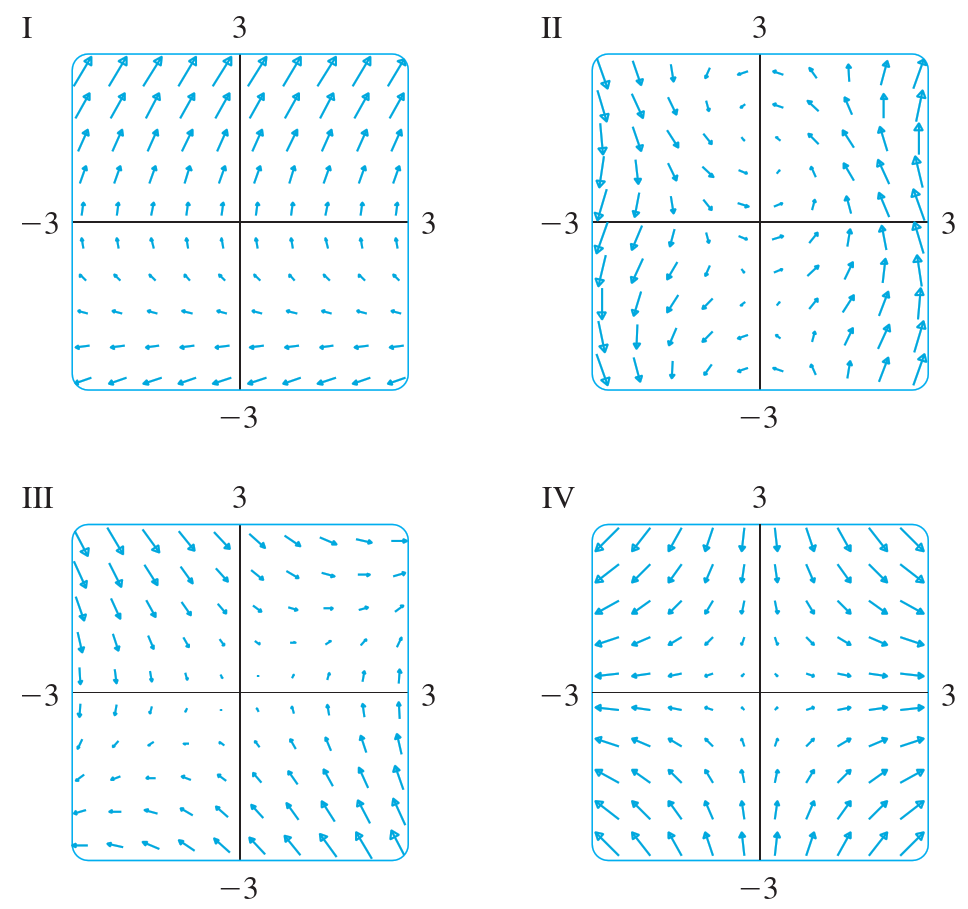
\includegraphics[width=\textwidth]{lista-11-fig1.png}
    \end{minipage}

    %\item Uma part\'{\i}cula se move em um campo de velocidade $V(x,y)=(x^2,x+y^2)$.
    %Se ela est\'a na posi\c{c}\~ao $(2,1)$ no instante $t=3$, estime sua posi\c{c}\~ao no
    %instante $t=3,01$.

    \item Calcule as integrais de linha.
        \begin{enumerate}
            \setlength\itemsep{0.2cm}
            \item $\ds\int_C y^3\ ds$, $C: x=t^3, y=t, 0\le t\le 2$
            \item $\ds\int_C xy^4\ ds$, $C$ \'e a metade direita do c\'{\i}rculo $x^2+y^2=16$
            \item $\ds\int_C x^2y^3-\sqrt{x}\ dy$, $C$ \'e o arco da curva
            $y=\sqrt{x}$ de $(1,1)$ a $(4,2)$
            \item $\ds\int_C xe^y\ dx$, $C$ \'e o arco da curva $x=e^y$ de
            $(1,0)$ a $(e,1)$
            \item $\ds\int_C z^2\ dx + x^2\ dy + y^2\ dz$, $C$ consiste no
            segmento de reta de $(1,0,0)$ a $(4,1,2)$
        \end{enumerate}

\end{enumerate}

\end{document}
